%%%% Paramétrage du TD %%%%
\def\xxactivite{ \ifprof \normalsize{Application 2 -- Corrigé } \else  Application 2 \fi} % \normalsize \vspace{-.4cm}
\def\xxauteur{\textsl{Xavier Pessoles}}


\def\xxnumchapitre{Chapitre 1 \vspace{.2cm}}
\def\xxchapitre{\hspace{.12cm} Équilibrage des solides en rotation}

\def\xxcompetences{%
%\textsl{%
%\textbf{Savoirs et compétences :}\\
%\begin{itemize}[label=\ding{112},font=\color{ocre}] 
%\item \textit{Res1.C2} : principe fondamental de la dynamique;
%\item \textit{Res1.C1.SF1} : proposer une démarche permettant la détermination de la loi de mouvement.
%\end{itemize}
%}
}

\def\xxtitreexo{Application 02}
\def\xxsourceexo{\hspace{.2cm} \footnotesize{Pôle Chateaubriand -- Joliot Curie}}

\def\xxfigures{
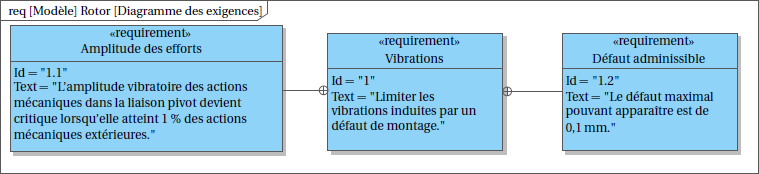
\includegraphics[width=.45\linewidth]{fig_01}
}%figues de la page de garde


\iflivret
\pagestyle{empty}


%%%%%%%% PAGE DE GARDE COURS
\ifcours
% ==== BANDEAU DES TITRES ==== 
\begin{tikzpicture}[remember picture,overlay]
\node at (current page.north west)
{\begin{tikzpicture}[remember picture,overlay]
\node[anchor=north west,inner sep=0pt] at (0,0) {\includegraphics[width=\paperwidth]{\thechapterimage}};
\draw[anchor=west] (-2cm,-8cm) node [line width=2pt,rounded corners=15pt,draw=ocre,fill=white,fill opacity=0.6,inner sep=40pt]{\strut\makebox[22cm]{}};
\draw[anchor=west] (1cm,-8cm) node {\huge\sffamily\bfseries\color{black} %
\begin{minipage}{1cm}
\rotatebox{90}{\LARGE\sffamily\textsc{\color{ocre}\textbf{\xxnumpartie}}}
\end{minipage} \hfill
\begin{minipage}[c]{14cm}
\begin{titrepartie}
\begin{flushright}
\renewcommand{\baselinestretch}{1.1} 
\Large\sffamily\textsc{\textbf{\xxpartie}}
\renewcommand{\baselinestretch}{1} 
\end{flushright}
\end{titrepartie}
\end{minipage} \hfill
\begin{minipage}[c]{3.5cm}
{\large\sffamily\textsc{\textbf{\color{ocre} \discipline}}}
\end{minipage} 
 };
\end{tikzpicture}};
\end{tikzpicture}
% ==== FIN BANDEAU DES TITRES ==== 


% ==== ONGLET 
\begin{tikzpicture}[overlay]
\node[shape=rectangle, 
      rounded corners = .25 cm,
	  draw= ocre,
	  line width=2pt, 
	  fill = ocre!10,
	  minimum width  = 2.5cm,
	  minimum height = 3cm,] at (18.3cm,0) {};
\node at (17.7cm,0) {\rotatebox{90}{\textbf{\Large\color{ocre}{\classe}}}};
%{};
\end{tikzpicture}
% ==== FIN ONGLET 


\vspace{3.5cm}

\begin{tikzpicture}[remember picture,overlay]
\draw[anchor=west] (-2cm,-6cm) node {\huge\sffamily\bfseries\color{black} %
\begin{minipage}{2cm}
\begin{center}
\LARGE\sffamily\textsc{\color{ocre}\textbf{\xxactivite}}
\end{center}
\end{minipage} \hfill
\begin{minipage}[c]{15cm}
\begin{titrechapitre}
\renewcommand{\baselinestretch}{1.1} 
\Large\sffamily\textsc{\textbf{\xxnumchapitre}}

\Large\sffamily\textsc{\textbf{\xxchapitre}}
\vspace{.5cm}

\renewcommand{\baselinestretch}{1} 
\normalsize\normalfont
\xxcompetences
\end{titrechapitre}
\end{minipage}  };
\end{tikzpicture}
\vfill

\begin{flushright}
\begin{minipage}[c]{.3\linewidth}
\begin{center}
\xxfigures
\end{center}
\end{minipage}\hfill
\begin{minipage}[c]{.6\linewidth}
\startcontents
%\printcontents{}{1}{}
\printcontents{}{1}{}
\end{minipage}
\end{flushright}

\begin{tikzpicture}[remember picture,overlay]
\draw[anchor=west] (4.5cm,-.7cm) node {
\begin{minipage}[c]{.2\linewidth}
\begin{flushright}

\includegraphics[width=2cm]{logoCC}
\end{flushright}
\end{minipage}
\begin{minipage}[c]{.2\linewidth}
\textsl{\xxauteur} \\
\textsl{\classe}
\end{minipage}
 };
\end{tikzpicture}

\newpage
\pagestyle{fancy}

%\newpage
%\pagestyle{fancy}

\else
\fi
%% FIN PAGE DE GARDE DES COURS

%%%%%%%% PAGE DE GARDE TD
\iftd
%\begin{tikzpicture}[remember picture,overlay]
%\node at (current page.north west)
%{\begin{tikzpicture}[remember picture,overlay]
%\draw[anchor=west] (-2cm,-3.25cm) node [line width=2pt,rounded corners=15pt,draw=ocre,fill=white,fill opacity=0.6,inner sep=40pt]{\strut\makebox[22cm]{}};
%\draw[anchor=west] (1cm,-3.25cm) node {\huge\sffamily\bfseries\color{black} %
%\begin{minipage}{1cm}
%\rotatebox{90}{\LARGE\sffamily\textsc{\color{ocre}\textbf{\xxnumpartie}}}
%\end{minipage} \hfill
%\begin{minipage}[c]{13.5cm}
%\begin{titrepartie}
%\begin{flushright}
%\renewcommand{\baselinestretch}{1.1} 
%\Large\sffamily\textsc{\textbf{\xxpartie}}
%\renewcommand{\baselinestretch}{1} 
%\end{flushright}
%\end{titrepartie}
%\end{minipage} \hfill
%\begin{minipage}[c]{3.5cm}
%{\large\sffamily\textsc{\textbf{\color{ocre} \discipline}}}
%\end{minipage} 
% };
%\end{tikzpicture}};
%\end{tikzpicture}

%%%%%%%%%% PAGE DE GARDE TD %%%%%%%%%%%%%%%
%\begin{tikzpicture}[overlay]
%\node[shape=rectangle, 
%      rounded corners = .25 cm,
%	  draw= ocre,
%	  line width=2pt, 
%	  fill = ocre!10,
%	  minimum width  = 2.5cm,
%	  minimum height = 2.5cm,] at (18.5cm,0) {};
%\node at (17.7cm,0) {\rotatebox{90}{\textbf{\Large\color{ocre}{\classe}}}};
%%{};
%\end{tikzpicture}

% PARTIE ET CHAPITRE
%\begin{tikzpicture}[remember picture,overlay]
%\draw[anchor=west] (-1cm,-2.1cm) node {\large\sffamily\bfseries\color{black} %
%\begin{minipage}[c]{15cm}
%\begin{flushleft}
%\xxnumchapitre \\
%\xxchapitre
%\end{flushleft}
%\end{minipage}  };
%\end{tikzpicture}

% BANDEAU EXO
\iflivret % SI LIVRET
\begin{tikzpicture}[remember picture,overlay]
\draw[anchor=west] (-2cm,-3.3cm) node {\huge\sffamily\bfseries\color{black} %
\begin{minipage}{5cm}
\begin{center}
\LARGE\sffamily\color{ocre}\textbf{\textsc{\xxactivite}}

\begin{center}
\xxfigures
\end{center}

\end{center}
\end{minipage} \hfill
\begin{minipage}[c]{12cm}
\begin{titrechapitre}
\renewcommand{\baselinestretch}{1.1} 
\large\sffamily\textbf{\textsc{\xxtitreexo}}

\small\sffamily{\textbf{\textit{\color{black!70}\xxsourceexo}}}
\vspace{.5cm}

\renewcommand{\baselinestretch}{1} 
\normalsize\normalfont
\xxcompetences
\end{titrechapitre}
\end{minipage}};
\end{tikzpicture}
\else % ELSE NOT LIVRET
\begin{tikzpicture}[remember picture,overlay]
\draw[anchor=west] (-2cm,-4.5cm) node {\huge\sffamily\bfseries\color{black} %
\begin{minipage}{5cm}
\begin{center}
\LARGE\sffamily\color{ocre}\textbf{\textsc{\xxactivite}}

\begin{center}
\xxfigures
\end{center}

\end{center}
\end{minipage} \hfill
\begin{minipage}[c]{12cm}
\begin{titrechapitre}
\renewcommand{\baselinestretch}{1.1} 
\large\sffamily\textbf{\textsc{\xxtitreexo}}

\small\sffamily{\textbf{\textit{\color{black!70}\xxsourceexo}}}
\vspace{.5cm}

\renewcommand{\baselinestretch}{1} 
\normalsize\normalfont
\xxcompetences
\end{titrechapitre}
\end{minipage}};
\end{tikzpicture}

\fi

\else   % FIN IF TD
\fi


%%%%%%%% PAGE DE GARDE FICHE
\iffiche
\begin{tikzpicture}[remember picture,overlay]
\node at (current page.north west)
{\begin{tikzpicture}[remember picture,overlay]
\draw[anchor=west] (-2cm,-2.25cm) node [line width=2pt,rounded corners=15pt,draw=ocre,fill=white,fill opacity=0.6,inner sep=40pt]{\strut\makebox[22cm]{}};
\draw[anchor=west] (1cm,-2.25cm) node {\huge\sffamily\bfseries\color{black} %
\begin{minipage}{1cm}
\rotatebox{90}{\LARGE\sffamily\textsc{\color{ocre}\textbf{\xxnumpartie}}}
\end{minipage} \hfill
\begin{minipage}[c]{14cm}
\begin{titrepartie}
\begin{flushright}
\renewcommand{\baselinestretch}{1.1} 
\large\sffamily\textsc{\textbf{\xxpartie} \\} 

\vspace{.2cm}

\normalsize\sffamily\textsc{\textbf{\xxnumchapitre -- \xxchapitre}}
\renewcommand{\baselinestretch}{1} 
\end{flushright}
\end{titrepartie}
\end{minipage} \hfill
\begin{minipage}[c]{3.5cm}
{\large\sffamily\textsc{\textbf{\color{ocre} \discipline}}}
\end{minipage} 
 };
\end{tikzpicture}};
\end{tikzpicture}

\iflivret
\begin{tikzpicture}[overlay]
\node[shape=rectangle, 
      rounded corners = .25 cm,
	  draw= ocre,
	  line width=2pt, 
	  fill = ocre!10,
	  minimum width  = 2.5cm,
	  minimum height = 2.5cm,] at (18.5cm,1.1cm) {};
\node at (17.9cm,1.1cm) {\rotatebox{90}{\textsf{\textbf{\large\color{ocre}{\classe}}}}};
%{};
\end{tikzpicture}
\else
\begin{tikzpicture}[overlay]
\node[shape=rectangle, 
      rounded corners = .25 cm,
	  draw= ocre,
	  line width=2pt, 
	  fill = ocre!10,
	  minimum width  = 2.5cm,
%	  minimum height = 2.5cm,] at (18.5cm,1.1cm) {};
	  minimum height = 2.5cm,] at (18.6cm,0cm) {};
\node at (18cm,0cm) {\rotatebox{90}{\textsf{\textbf{\large\color{ocre}{\classe}}}}};
%{};
\end{tikzpicture}

\fi

\else
\fi



\else
\pagestyle{empty}


%%%%%%%% PAGE DE GARDE COURS
\ifcours
% ==== BANDEAU DES TITRES ==== 
\begin{tikzpicture}[remember picture,overlay]
\node at (current page.north west)
{\begin{tikzpicture}[remember picture,overlay]
\node[anchor=north west,inner sep=0pt] at (0,0) {\includegraphics[width=\paperwidth]{\thechapterimage}};
\draw[anchor=west] (-2cm,-8cm) node [line width=2pt,rounded corners=15pt,draw=ocre,fill=white,fill opacity=0.6,inner sep=40pt]{\strut\makebox[22cm]{}};
\draw[anchor=west] (1cm,-8cm) node {\huge\sffamily\bfseries\color{black} %
\begin{minipage}{1cm}
\rotatebox{90}{\LARGE\sffamily\textsc{\color{ocre}\textbf{\xxnumpartie}}}
\end{minipage} \hfill
\begin{minipage}[c]{14cm}
\begin{titrepartie}
\begin{flushright}
\renewcommand{\baselinestretch}{1.1} 
\Large\sffamily\textsc{\textbf{\xxpartie}}
\renewcommand{\baselinestretch}{1} 
\end{flushright}
\end{titrepartie}
\end{minipage} \hfill
\begin{minipage}[c]{3.5cm}
{\large\sffamily\textsc{\textbf{\color{ocre} \discipline}}}
\end{minipage} 
 };
\end{tikzpicture}};
\end{tikzpicture}
% ==== FIN BANDEAU DES TITRES ==== 


% ==== ONGLET 
\begin{tikzpicture}[overlay]
\node[shape=rectangle, 
      rounded corners = .25 cm,
	  draw= ocre,
	  line width=2pt, 
	  fill = ocre!10,
	  minimum width  = 2.5cm,
	  minimum height = 3cm,] at (18.3cm,0) {};
\node at (17.7cm,0) {\rotatebox{90}{\textbf{\Large\color{ocre}{\classe}}}};
%{};
\end{tikzpicture}
% ==== FIN ONGLET 


\vspace{3.5cm}

\begin{tikzpicture}[remember picture,overlay]
\draw[anchor=west] (-2cm,-6cm) node {\huge\sffamily\bfseries\color{black} %
\begin{minipage}{2cm}
\begin{center}
\LARGE\sffamily\textsc{\color{ocre}\textbf{\xxactivite}}
\end{center}
\end{minipage} \hfill
\begin{minipage}[c]{15cm}
\begin{titrechapitre}
\renewcommand{\baselinestretch}{1.1} 
\Large\sffamily\textsc{\textbf{\xxnumchapitre}}

\Large\sffamily\textsc{\textbf{\xxchapitre}}
\vspace{.5cm}

\renewcommand{\baselinestretch}{1} 
\normalsize\normalfont
\xxcompetences
\end{titrechapitre}
\end{minipage}  };
\end{tikzpicture}
\vfill

\begin{flushright}
\begin{minipage}[c]{.3\linewidth}
\begin{center}
\xxfigures
\end{center}
\end{minipage}\hfill
\begin{minipage}[c]{.6\linewidth}
\startcontents
%\printcontents{}{1}{}
\printcontents{}{1}{}
\end{minipage}
\end{flushright}

\begin{tikzpicture}[remember picture,overlay]
\draw[anchor=west] (4.5cm,-.7cm) node {
\begin{minipage}[c]{.2\linewidth}
\begin{flushright}

\includegraphics[width=2cm]{logoCC}
\end{flushright}
\end{minipage}
\begin{minipage}[c]{.2\linewidth}
\textsl{\xxauteur} \\
\textsl{\classe}
\end{minipage}
 };
\end{tikzpicture}

\newpage
\pagestyle{fancy}

%\newpage
%\pagestyle{fancy}

\else
\fi
%% FIN PAGE DE GARDE DES COURS

%%%%%%%% PAGE DE GARDE TD
\iftd
%\begin{tikzpicture}[remember picture,overlay]
%\node at (current page.north west)
%{\begin{tikzpicture}[remember picture,overlay]
%\draw[anchor=west] (-2cm,-3.25cm) node [line width=2pt,rounded corners=15pt,draw=ocre,fill=white,fill opacity=0.6,inner sep=40pt]{\strut\makebox[22cm]{}};
%\draw[anchor=west] (1cm,-3.25cm) node {\huge\sffamily\bfseries\color{black} %
%\begin{minipage}{1cm}
%\rotatebox{90}{\LARGE\sffamily\textsc{\color{ocre}\textbf{\xxnumpartie}}}
%\end{minipage} \hfill
%\begin{minipage}[c]{13.5cm}
%\begin{titrepartie}
%\begin{flushright}
%\renewcommand{\baselinestretch}{1.1} 
%\Large\sffamily\textsc{\textbf{\xxpartie}}
%\renewcommand{\baselinestretch}{1} 
%\end{flushright}
%\end{titrepartie}
%\end{minipage} \hfill
%\begin{minipage}[c]{3.5cm}
%{\large\sffamily\textsc{\textbf{\color{ocre} \discipline}}}
%\end{minipage} 
% };
%\end{tikzpicture}};
%\end{tikzpicture}

%%%%%%%%%% PAGE DE GARDE TD %%%%%%%%%%%%%%%
%\begin{tikzpicture}[overlay]
%\node[shape=rectangle, 
%      rounded corners = .25 cm,
%	  draw= ocre,
%	  line width=2pt, 
%	  fill = ocre!10,
%	  minimum width  = 2.5cm,
%	  minimum height = 2.5cm,] at (18.5cm,0) {};
%\node at (17.7cm,0) {\rotatebox{90}{\textbf{\Large\color{ocre}{\classe}}}};
%%{};
%\end{tikzpicture}

% PARTIE ET CHAPITRE
%\begin{tikzpicture}[remember picture,overlay]
%\draw[anchor=west] (-1cm,-2.1cm) node {\large\sffamily\bfseries\color{black} %
%\begin{minipage}[c]{15cm}
%\begin{flushleft}
%\xxnumchapitre \\
%\xxchapitre
%\end{flushleft}
%\end{minipage}  };
%\end{tikzpicture}

% BANDEAU EXO
\iflivret % SI LIVRET
\begin{tikzpicture}[remember picture,overlay]
\draw[anchor=west] (-2cm,-3.3cm) node {\huge\sffamily\bfseries\color{black} %
\begin{minipage}{5cm}
\begin{center}
\LARGE\sffamily\color{ocre}\textbf{\textsc{\xxactivite}}

\begin{center}
\xxfigures
\end{center}

\end{center}
\end{minipage} \hfill
\begin{minipage}[c]{12cm}
\begin{titrechapitre}
\renewcommand{\baselinestretch}{1.1} 
\large\sffamily\textbf{\textsc{\xxtitreexo}}

\small\sffamily{\textbf{\textit{\color{black!70}\xxsourceexo}}}
\vspace{.5cm}

\renewcommand{\baselinestretch}{1} 
\normalsize\normalfont
\xxcompetences
\end{titrechapitre}
\end{minipage}};
\end{tikzpicture}
\else % ELSE NOT LIVRET
\begin{tikzpicture}[remember picture,overlay]
\draw[anchor=west] (-2cm,-4.5cm) node {\huge\sffamily\bfseries\color{black} %
\begin{minipage}{5cm}
\begin{center}
\LARGE\sffamily\color{ocre}\textbf{\textsc{\xxactivite}}

\begin{center}
\xxfigures
\end{center}

\end{center}
\end{minipage} \hfill
\begin{minipage}[c]{12cm}
\begin{titrechapitre}
\renewcommand{\baselinestretch}{1.1} 
\large\sffamily\textbf{\textsc{\xxtitreexo}}

\small\sffamily{\textbf{\textit{\color{black!70}\xxsourceexo}}}
\vspace{.5cm}

\renewcommand{\baselinestretch}{1} 
\normalsize\normalfont
\xxcompetences
\end{titrechapitre}
\end{minipage}};
\end{tikzpicture}

\fi

\else   % FIN IF TD
\fi


%%%%%%%% PAGE DE GARDE FICHE
\iffiche
\begin{tikzpicture}[remember picture,overlay]
\node at (current page.north west)
{\begin{tikzpicture}[remember picture,overlay]
\draw[anchor=west] (-2cm,-2.25cm) node [line width=2pt,rounded corners=15pt,draw=ocre,fill=white,fill opacity=0.6,inner sep=40pt]{\strut\makebox[22cm]{}};
\draw[anchor=west] (1cm,-2.25cm) node {\huge\sffamily\bfseries\color{black} %
\begin{minipage}{1cm}
\rotatebox{90}{\LARGE\sffamily\textsc{\color{ocre}\textbf{\xxnumpartie}}}
\end{minipage} \hfill
\begin{minipage}[c]{14cm}
\begin{titrepartie}
\begin{flushright}
\renewcommand{\baselinestretch}{1.1} 
\large\sffamily\textsc{\textbf{\xxpartie} \\} 

\vspace{.2cm}

\normalsize\sffamily\textsc{\textbf{\xxnumchapitre -- \xxchapitre}}
\renewcommand{\baselinestretch}{1} 
\end{flushright}
\end{titrepartie}
\end{minipage} \hfill
\begin{minipage}[c]{3.5cm}
{\large\sffamily\textsc{\textbf{\color{ocre} \discipline}}}
\end{minipage} 
 };
\end{tikzpicture}};
\end{tikzpicture}

\iflivret
\begin{tikzpicture}[overlay]
\node[shape=rectangle, 
      rounded corners = .25 cm,
	  draw= ocre,
	  line width=2pt, 
	  fill = ocre!10,
	  minimum width  = 2.5cm,
	  minimum height = 2.5cm,] at (18.5cm,1.1cm) {};
\node at (17.9cm,1.1cm) {\rotatebox{90}{\textsf{\textbf{\large\color{ocre}{\classe}}}}};
%{};
\end{tikzpicture}
\else
\begin{tikzpicture}[overlay]
\node[shape=rectangle, 
      rounded corners = .25 cm,
	  draw= ocre,
	  line width=2pt, 
	  fill = ocre!10,
	  minimum width  = 2.5cm,
%	  minimum height = 2.5cm,] at (18.5cm,1.1cm) {};
	  minimum height = 2.5cm,] at (18.6cm,0cm) {};
\node at (18cm,0cm) {\rotatebox{90}{\textsf{\textbf{\large\color{ocre}{\classe}}}}};
%{};
\end{tikzpicture}

\fi

\else
\fi



\fi
\setlength{\columnseprule}{.1pt}

\pagestyle{fancy}
\thispagestyle{plain}

\ifprof
\vspace{5.5cm}
\else
\vspace{4.9cm}
\fi

\def\columnseprulecolor{\color{ocre}}
\setlength{\columnseprule}{0.4pt} 

%%%%%%%%%%%%%%%%%%%%%%%

\setcounter{exo}{0}

\ifprof
\else

\begin{multicols}{2}

\subsection*{Présentation}

On s’intéresse à une centrifugeuse humaine dont on donne une description structurelle ainsi que la
modélisation cinématique.
Le système étudié est constitué de 4 éléments principaux :
\begin{itemize}
\item un massif-bâti en béton 0 sur lequel est rigidement ancré un axe assurant le guidage en rotation du sous ensemble 1
autour d’un axe vertical ;
\item un sous ensemble 1 en rotation autour de l’axe vertical qui est composé d’un contrepoids $c$, d’une virole $v$ et d’un bras en treillis tubulaire $b$;
\item un anneau 2, interposé entre la nacelle et le bras, autorisant les rotations autour des 2 axes orthogonaux (roulis et tangage) ;
\item une nacelle instrumentée 3 équipée du siège pour le pilote.
\end{itemize}

\begin{center}
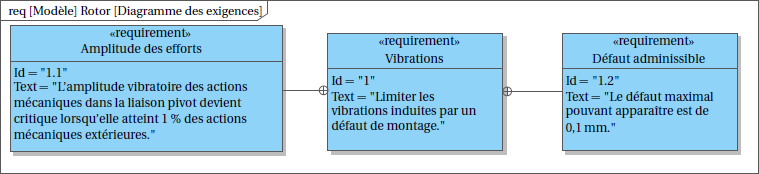
\includegraphics[width=\linewidth]{fig_01.png}
\end{center}

Aux 4 éléments précédents s’ajoutent des équipements complémentaires : un générateur de puissance
hydraulique, un réducteur pouvant transmettre une puissance de l’ordre de \SI{1}{MW} pour le mouvement de
rotation du sous ensemble 1 par rapport à 0, une motorisation embarquée pour les mouvements de rotation
de roulis et de tangage, un système d’asservissement pour chaque actionneur.

Cette conception permet de lier de façon univoque, les profils de position (ou de vitesse relative) engendrés
au niveau de chaque liaison à l’évolution temporelle des 3 composantes d’accélération que subit le pilote.
Ainsi les consignes de position ou de vitesse à appliquer aux liaisons sont directement déduites de
l’accélération à reproduire. La vitesse de rotation du bras détermine l’intensité de l’accélération imposée au
pilote et l’orientation de la nacelle en roulis et tangage fixe la direction de l’accélération imposée au pilote.

\subsection*{Modélisation cinématique et paramétrage}
\begin{center}
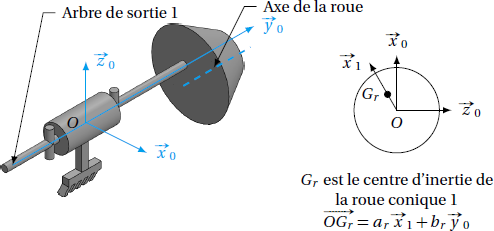
\includegraphics[width=\linewidth]{fig_02.png}
\end{center}

À l'arrêt les angles $\alpha$ et $\theta$ sont nuls.

\begin{itemize}
\item Le repère $\rep{0}=\repere{O}{x_0}{y_0}{z_0}$ est lié au bâti 0. Ce repère sera considéré comme galiléen. Le champ de la pesanteur est défini par $\vect{g}=g\vect{z_0}$.
\item Le repère $\rep{1}=\repere{O}{x_1}{y_1}{z_0}$ est lié au sous ensemble 1 (composée du contrepoids c, de la virole v et du bras en treillis tubulaire b). La liaison 1/0 est considérée comme une liaison pivot parfaite d’axe $\axe{O}{z_0}$, sa position est paramétrée par l’angle $\psi(t)=\angl{x_0}{x_1}$.
\item Le repère $\rep{2}=\repere{O}{x_1}{y_2}{z_2}$ est lié à l'anneau 2. La liaison 2/1 est considérée comme une liaison pivot parfaite d’axe $\axe{C}{x_1}$, sa position est paramétrée par l’angle $\theta(t)=\angl{y_1}{y_2}$. $\theta$ est appelé angle de roulis, la position du point $C$ est définie par le vecteur $\vect{OC}=-R\vect{y_1}$ avec $R=\SI{7,62}{m}$. 
\item Le repère $\rep{3}=\repere{C}{x_3}{y_2}{z_3}$ est lié à la nacelle 3 dans laquelle le pilote prend place. La liaison 3/2 est considérée comme une liaison pivot parfaite d’axe $\axe{C}{y_2}$, sa position est paramétrée par l’angle $\alpha(t)=\angl{x_2}{x_3}$.
\end{itemize}

\subsection*{Géométrie des masses}
Les valeurs approchées des moments d’inertie suivants ne sont données qu’à titre indicatif. Le sous ensemble (1) est composé de la virole v, du contrepoids c et du bras b. 

\begin{center}
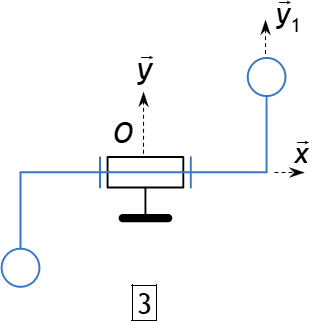
\includegraphics[width=\linewidth]{fig_03.png}
\end{center}


\textbf{Sous ensemble (1)}
\begin{itemize}
\item Virole : masse $m_v=\SI{8325}{kg}$, centre de gravité 
$G_v$ tel que $\vect{OG_v}=z_v\vect{z_0}$ avec $z_v=\SI{0,63}{m}$, matrice d'inertie $\inertie{O}{v}=\matinertie{A_v}{A_v}{C_v}{0}{0}{0}{\rep{1}}$, avec $A_v=\SI{20625}{kg.m^2}$ et $C_v=\SI{17600}{kg.m^2}$.
\item Contrepoids : masse $m_c=\SI{5600}{kg}$, centre de gravité 
$G_c$ tel que $\vect{OG_c}=y_c\vect{y_1}$ avec $y_c=\SI{2}{m}$, matrice d'inertie $\inertie{O}{c}=\matinertie{A_c}{B_c}{C_c}{0}{0}{0}{\rep{1}}$, avec $A_c=\SI{25625}{kg.m^2}$, $B_c=\SI{3000}{kg.m^2}$ et $C_c=\SI{22775}{kg.m^2}$.
\item Bras: masse $m_b=\SI{1980}{kg}$, centre de gravité 
$G_b$ tel que $\vect{OG_b}=-y_b\vect{y_1}$ avec $y_b=\SI{3,45}{m}$, matrice d'inertie $\inertie{O}{b}=\matinertie{A_b}{B_b}{C_b}{0}{0}{0}{\rep{1}}$, avec $A_b=\SI{31575}{kg.m^2}$, $B_b=\SI{6000}{kg.m^2}$ et $C_b=\SI{33775}{kg.m^2}$.
\end{itemize}

\textbf{Anneau (2)}
Masse et inertie supposées négligeables dans cette approche.


\textbf{Nacelle et pilote (3)}
\begin{itemize}
\item Masse $m_3=\SI{1705}{kg}$, le centre de gravité  reste confondu avec le point $C$ tel que $\vect{OC}=-R\vect{y_1}$ avec ${R}=\SI{7,62}{m}$, matrice d'inertie $\inertie{C}{3}=\matinertie{A_3}{B_3}{A_3}{0}{0}{0}{\repere{C}{x_3}{y_2}{z_3}\text{ et } \repere{C}{x_1}{y_2}{z_2}}$, avec $A_3=\SI{135}{kg.m^2}$ et $B_3=\SI{1575}{kg.m^2}$.
\end{itemize}


\subsection*{Étude des équilibrages statiques et dynamiques}
La centrifugeuse comporte, en complément de l’ensemble des éléments précédemment décrits, deux
contrepoids mobiles par rapport au sous-ensemble 1 et repérés 4 et 5. Ces contrepoids placés symétriquement
par rapport au plan $\left( O,\vect{y_1},\vect{z_0}\right)$ sont modélisés par des cylindres de révolution.

Les liaisons contrepoids 4/virole 1 et contrepoids 5/virole 1 sont assimilées à des liaisons glissières parfaites
de direction $\vect{z_0}$. Le schéma ci-dessous définit les implantations de ces deux contrepoids mobiles dans le repère
$\rep{1}$ ainsi que les notations complémentaires retenues pour la géométrie des masses.

\begin{center}
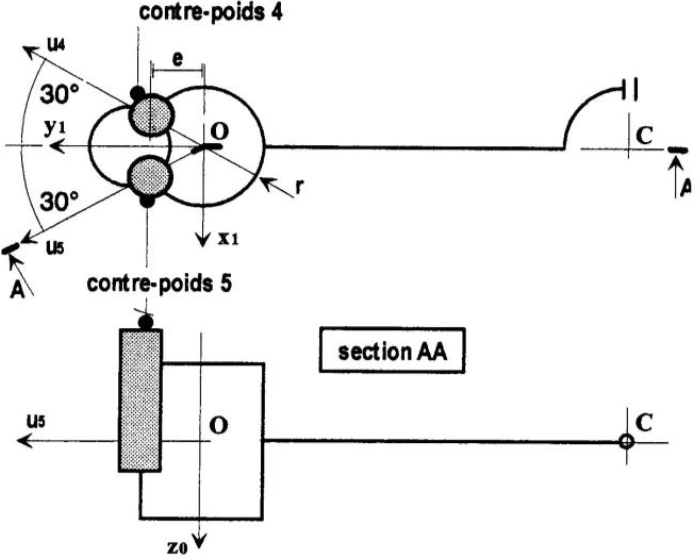
\includegraphics[width=\linewidth]{fig_04.png}
\end{center}


\textbf{Contrepoids mobile $i$ ($i=$ 4 ou 5)}
\begin{itemize}
\item Masse $m_i$, le centre de gravité $G_i$ est tel que $\vect{OG_i}=r\vect{u_i}+z_i \vect{z_0}$ et $\vect{OG_i}\vect{y_1}=e$  avec ${e}=\SI{1,2}{m}$, matrice d'inertie $\inertie{G_i}{i}=\matinertie{A_i}{A_i}{C_i}{0}{0}{0}{\repere{G_i}{x_1}{y_1}{z_0}}$.
\end{itemize}



\subparagraph{}
\textit{Quelle est la condition nécessaire afin de réaliser l’équilibrage statique de l’ensemble
$E$ en liaison pivot autour de l’axe $\axe{O}{z_0}$ avec le massif bâti 0 ? Exprimer les relations
traduisant cet équilibrage statique.
}
\ifprof
\begin{corrige}
\end{corrige}\else\fi


\subparagraph{}
\textit{En déduire l’expression des masses des deux contrepoids mobiles $m_4$ et $m_5$ en fonction des données du
problème. Faire l’application numérique. }
\ifprof
\begin{corrige}
\end{corrige}\else\fi


\subparagraph{}
\textit{Exprimer la coordonnée $z_G$ du centre de gravité de l’ensemble E en fonction de $z_4$ et $z_5$.}
\ifprof
\begin{corrige}
\end{corrige}\else\fi


\subparagraph{}
\textit{Exprimer de façon formelle les conditions qui traduisent l’équilibrage dynamique de l’ensemble $E$ en liaison pivot autour de l’axe $\axe{O}{z_0}$ avec le massif bâti 0 ? Quelles sont les conséquences de l’équilibrage dynamique sur la matrice d’inertie exprimée en $O$ de l’ensemble $E$ ? Donner la forme de cette matrice.}
\ifprof
\begin{corrige}
\end{corrige}\else\fi


\subparagraph{}
\textit{ En tenant compte des données du problème que peut-on dire de la forme de la matrice d’inertie du
sous ensemble 1 exprimée en $O$ dans la base $\base{x_1}{y_1}{z_0}$.}
\ifprof
\begin{corrige}
\end{corrige}\else\fi


\subparagraph{}
\textit{Déterminer la matrice la matrice d’inertie du solide 4 exprimée en $O$ dans la base $\base{x_1}{y_1}{z_0}$ en fonction $m_4$, $x_4$, $y_4$, $z_4$, $A_4$ et $C_4$.}
\ifprof
\begin{corrige}
\end{corrige}\else\fi


\subparagraph{}
\textit{En déduire la matrice la matrice d’inertie du solide 5 exprimée en $O$ dans la base $\base{x_1}{y_1}{z_0}$.
}
\ifprof
\begin{corrige}
\end{corrige}\else\fi


\subparagraph{}
\textit{Exprimer la matrice de passage notée $[P]$ de la base $\base{x_1}{y_2}{z_2}$ vers la base $\base{x_1}{y_1}{z_0}$ et en déduire la matrice d’inertie du solide 3 exprimée en $C$ dans la base $\base{x_1}{y_1}{z_0}$.}
\ifprof
\begin{corrige}
\end{corrige}\else\fi

\subparagraph{}
\textit{Déterminer les moments produits de la matrice d’inertie du solide 3 exprimée en $O$ dans la base $\base{x_1}{y_1}{z_0}$.}
\ifprof
\begin{corrige}
\end{corrige}\else\fi

\subparagraph{}
\textit{À partir des conditions d’équilibrage dynamique définies précédemment, déterminer les coordonnées
$z_4$ et $z_5$ des centres de gravité des contrepoids 4 et 5 en fonction de $A_3$, $B_3$ et $\theta$.
}
\ifprof
\begin{corrige}
\end{corrige}\else\fi

La conception de la centrifugeuse permet de lier les profils de position (ou de vitesse relative) engendrés au
niveau de chaque liaison à l’évolution temporelle des 3 composantes d’accélération que subit le pilote. Ainsi
comme la vitesse de rotation du bras détermine l’intensité de l’accélération imposée au pilote, la consigne
de position du roulis $\theta$ est liée à cette vitesse de rotation $\dot{\psi}$ du bras par la relation
$ \theta=\arctan\dfrac{R\dot{\psi}^2}{g}$. Lorsque le taux de rotation est a $\dot{\psi}=\SI{4,39}{rad/s}$ le pilote subit une accélération simulée de la pesanteur de $15g$.


\subparagraph{}
\textit{Déduire à partir des résultats de la question 10 les valeurs numériques de $z_4$ et $z_5$ lorsque le pilote
subit cette accélération simulée de la pesanteur de $15 g$.}

\end{multicols}

\fi

\ifprof

\begin{center}
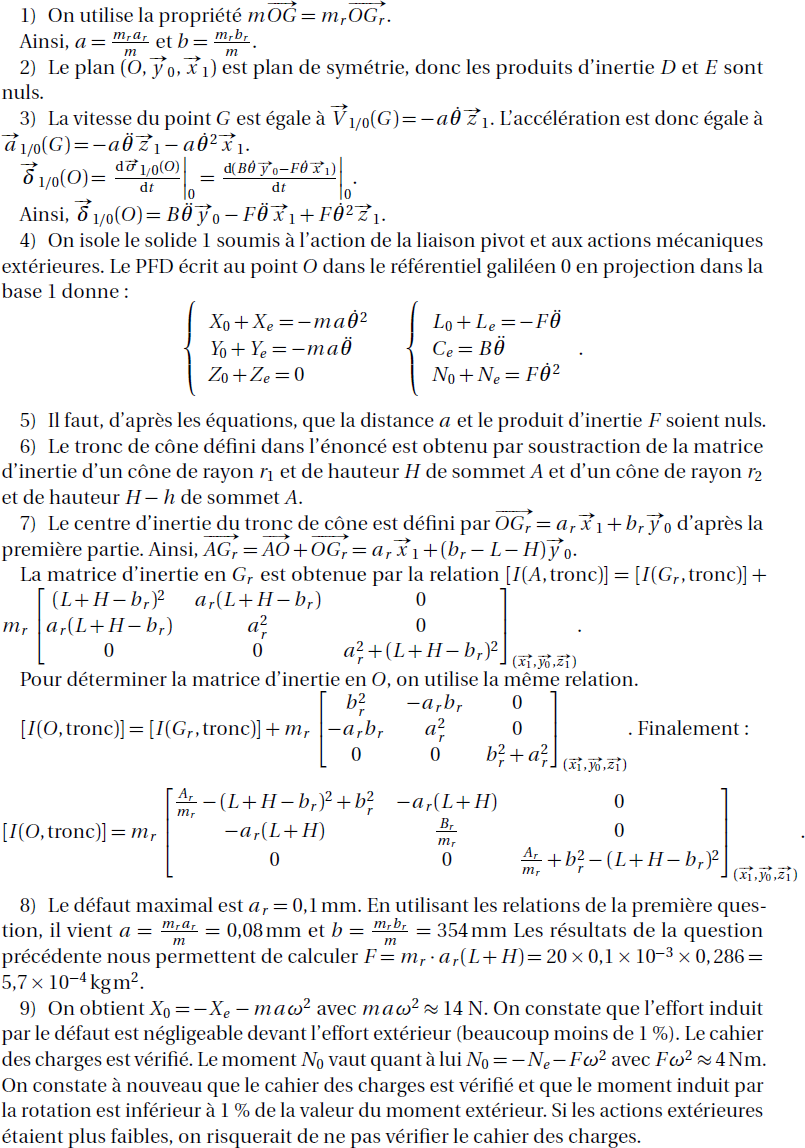
\includegraphics[width=\linewidth]{cor_01.png}
\end{center}
\begin{center}
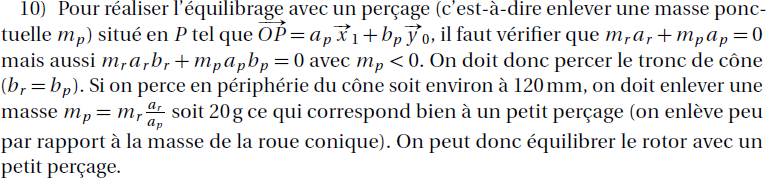
\includegraphics[width=\linewidth]{cor_02.png}
\end{center}
\begin{center}
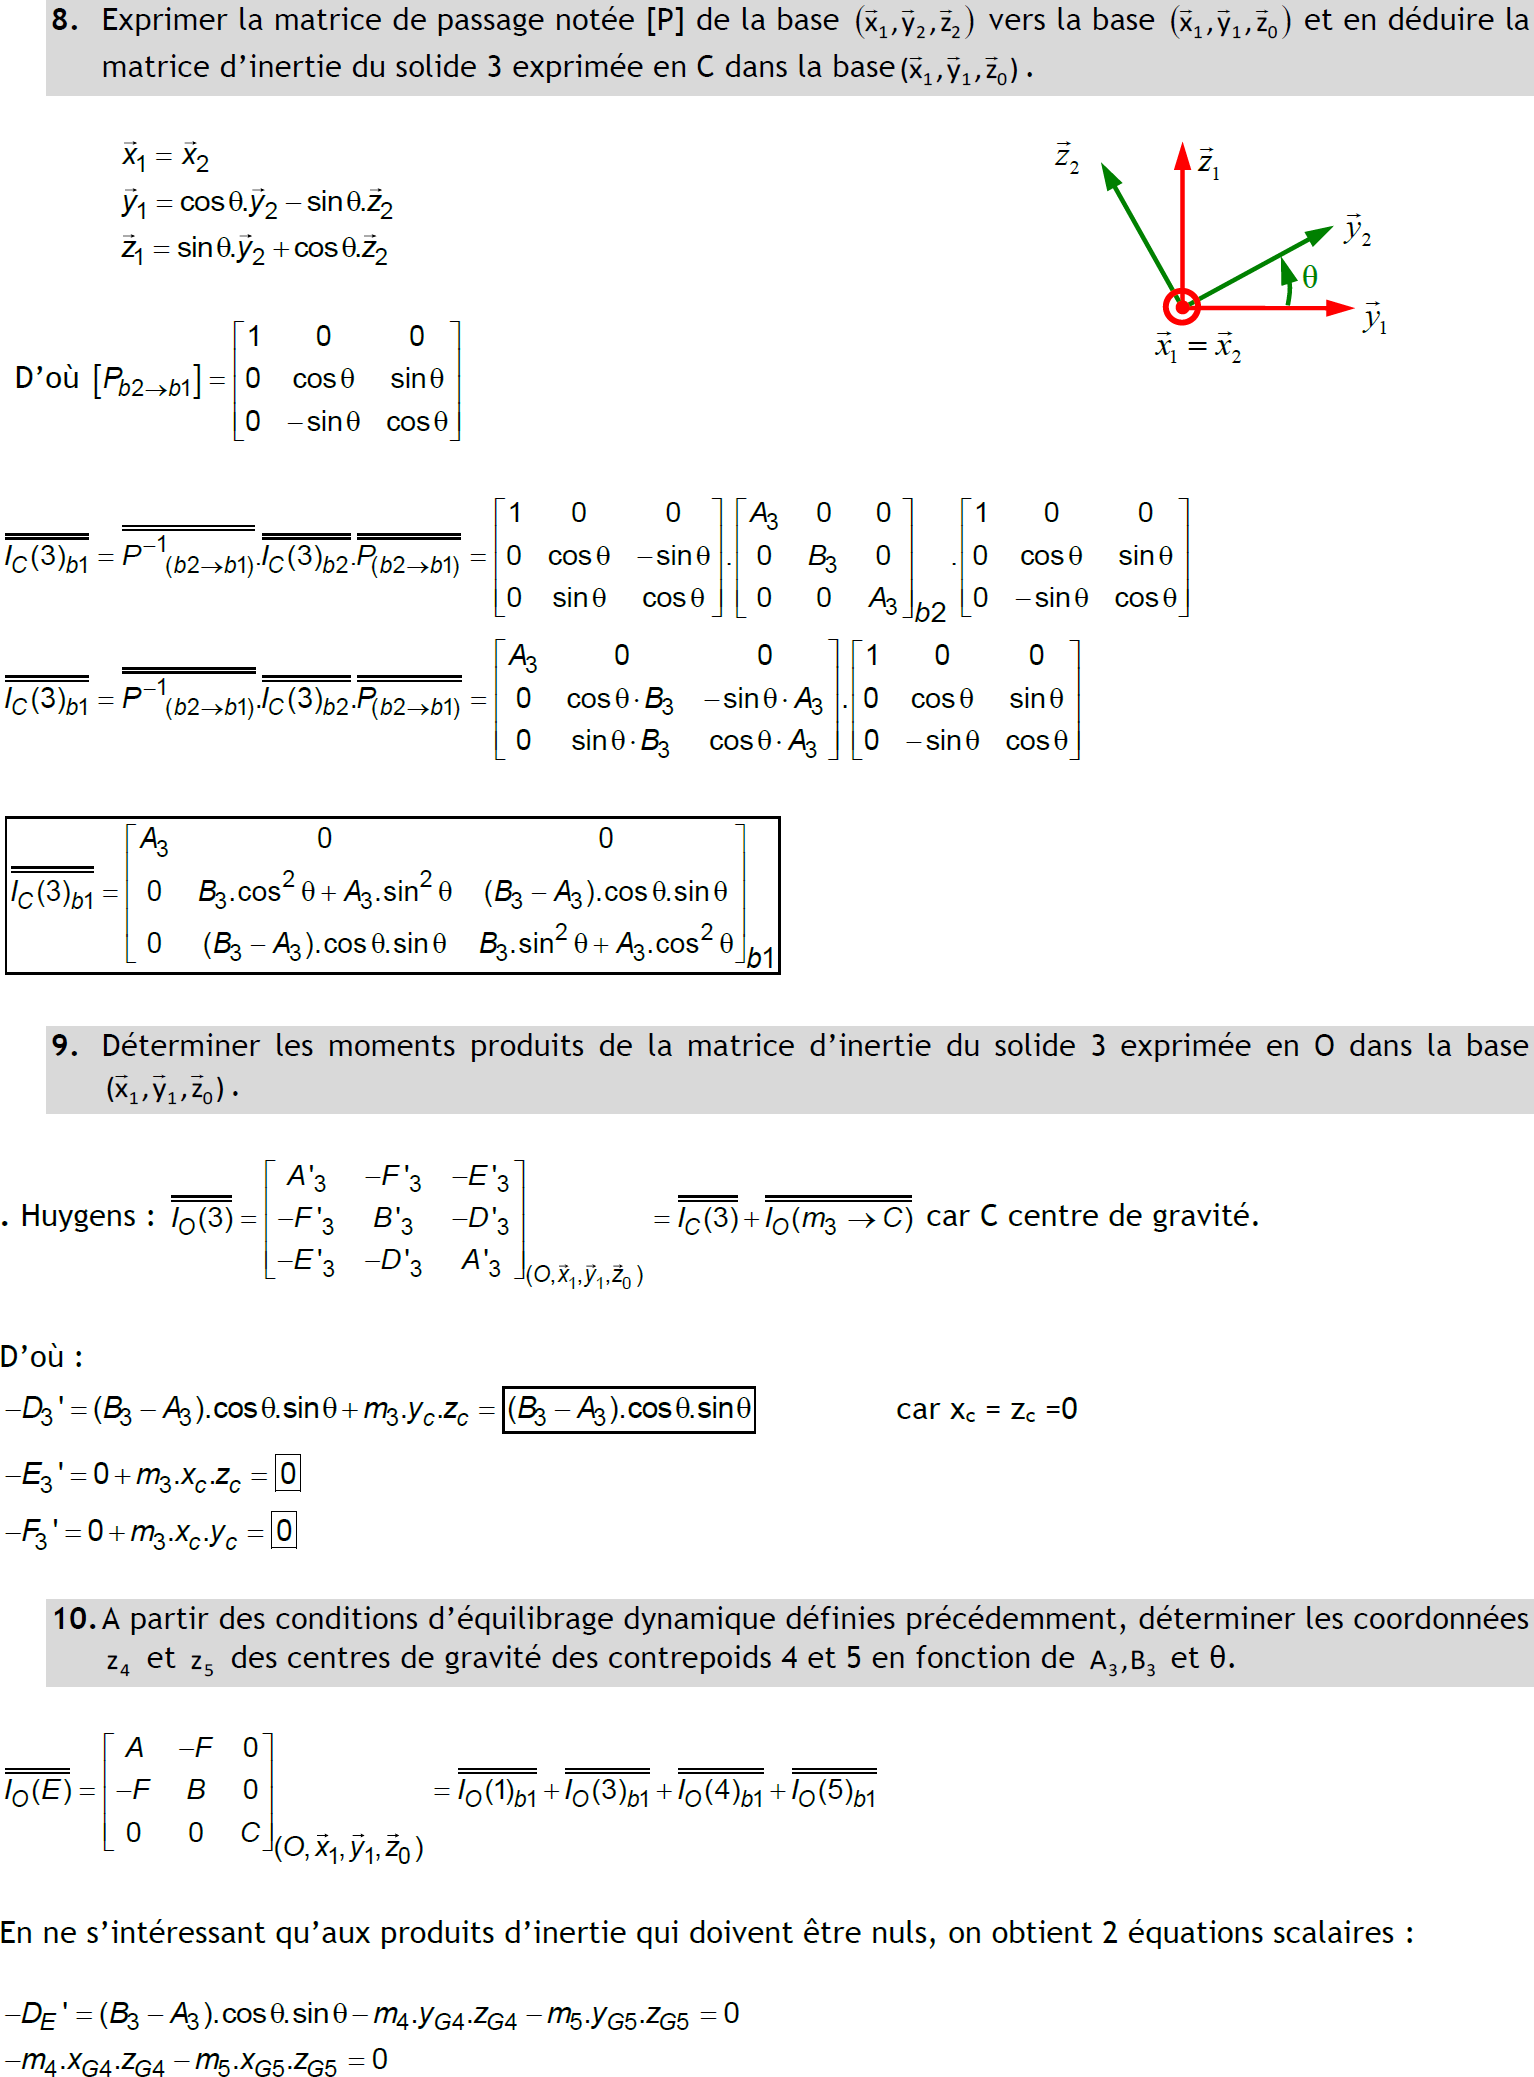
\includegraphics[width=\linewidth]{cor_03.png}
\end{center}
\begin{center}
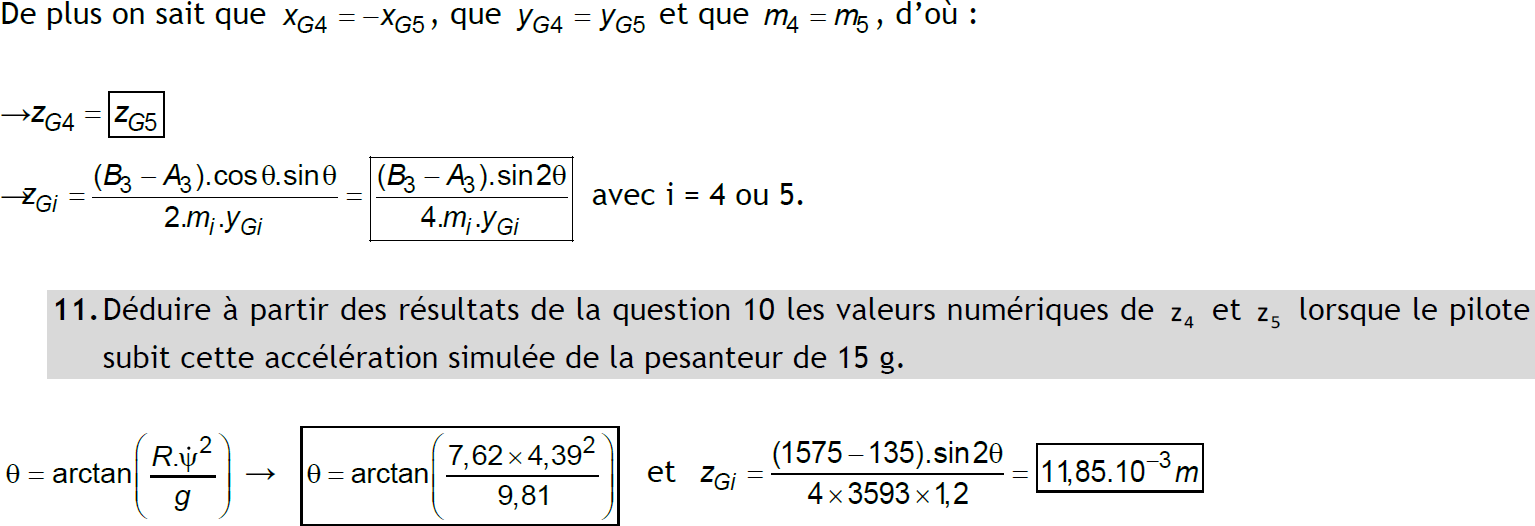
\includegraphics[width=\linewidth]{cor_04.png}
\end{center}
\else
\fi
